%!TEX root = ../thesis.tex
%*******************************************************************************
%*********************************** Fourth Chapter *****************************
%*******************************************************************************

\chapter{Evaluation}  %Title 

\ifpdf
    \graphicspath{{Chapters/Chapter4/Figs/Raster/}{Chapters/Chapter4/Figs/PDF/}{Chapters/Chapter4/Figs/}}
\else
    \graphicspath{{Chapters/Chapter4/Figs/Vector/}{Chapters/Chapter4/Figs/}}
\fi


%********************************** %First Section  **************************************
\section{Manual analysis of videos}

% TODO: add 'disappointing results' to the appendices

I initially tried to use Gaps directly as a feature for identifying foragers. This produced disappointing results and led me to believe there might be a mistake in the process. I felt the need to vaildate my steps so far and try a different value for the confidence threshold parameter (0.2 instead of 0.99). I refered to recordings from the hive as the best source of ground truth,
I randomly selected 200 Gaps (100 for each testet threshold value). I generated a two-minute video for each of them, with the moment the bee disappears placed in the middle of the video (subject to variation resulting from the closing operation - hence the 1min margin on each side). 


When analyzing the videos, I was trying to achieve a few goals:
\begin{itemize}
\item test which value of detection confidence threshold procuces better results
\item validate whether Presence and Gaps represent what they were designed to
\item draw general conclusions about the viability of this method for the forager problem
\item see first hand the difficulties and limitations
\end{itemize}

%TODO: emphasis (bold and italics)
In summary, I found that while Presence and Gaps seemed reliably defined and that the problem lay in the difficulty of defining Trips on top of Gaps.
%TODO: FIG: distribution of confidence values in detections from e.g. one given day). 

\section{Validating Presence}

On top of each video, I was displaying the output of my measures for Presence score and Presence binarized. Those were being updated at the beginning of each of the four 30-second intervals that the video contained. I was comparing these values to what I could observe in the videos myself. 

While my manual observations are obviously not perfectly quantifiable, I found that Presence scores corresponded to what I was seeing: intervals with perfect visibility of the tag had maximum scores and lower scores corresponded to proportionally lower observed visibility. The binarized value for presence was consistent with the score and the threshold, except for situations where it was changed by the morphological closing operator.


\section{Validating Gaps and their causes}


For every video, I was noting down:

\begin{itemize}
\item whether the bee really disappeared at that moment (as seen by a human observer)
\item the reason she disappeared 
\item whether the reason for her disappearance could be a foraging trip
\end{itemize}

Only a small number of Gaps turned out to be false positives, and that value was twice as low for a lower confidence threshold (0.2). This is a desired and interpretable result: a lower threshold means that more detections are taken into account. That makes it easier for the system to consider a bee present, which fills some Gaps that were created artificially and should not be there. It could also potentially create those artificial Gaps from misidentifying tags (and therefore seeing bees while they are not there) - but it seems like the system has more robustness against that, since the overall number of artificial gaps has decreased so significantly.

\begin{table}[h]
    % "Percentage of true positives in the gaps list, overall and by threshold
    \caption{Percentage of confirmable gaps by detection confidence threshold}
    \centering
    \label{table:conf_comparison}
    \begin{tabular}{@{}lccc@{}}
        \toprule
                       & High threshold (0.99) & Low threshold (0.2)  & Overall \\ \midrule
        Real gaps      & 88\%                & 94\%                  & 91\%    
    \end{tabular}
\end{table}

The number of Gaps that were not caused by a bee leaving the hive has far exceeded my expectations. To get a better understanging, I was noting the disappearance reason for all 200 videos I analyzed. Please keep in mind that with some complex interactions, it was difficult to name one, in which case I took the "top" one. For example, a bee migh be briefly occluded by crowd, and during that brief moment of invisibility hide permanently in a cell. The real reason she's not visible for the next few minutes is that she's in a cell, but neither I nor an automatic system of today's capabilities could pick up on that. A bee disappearing from the field of view of the camera is also just a proxy reason for something else - after all, she would be in the view of another camera and we could keep tracking her there.

\begin{figure}[htbp!] 
\centering
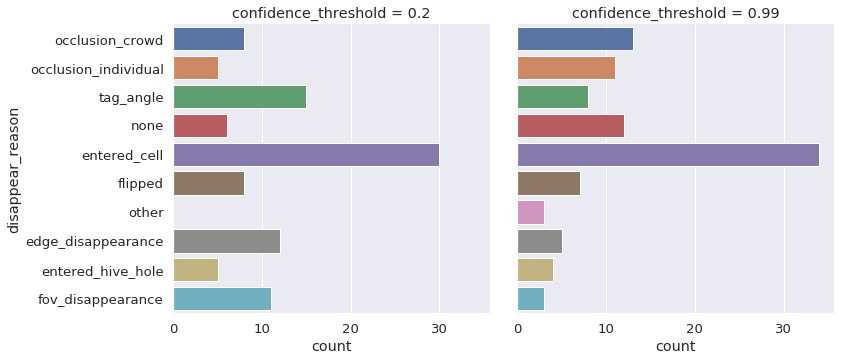
\includegraphics[width=1.0\textwidth]{gap-reason-dist}
\caption[gap-reason-dist]{Comparison of reasons a Gap has started, for two different values of confidence threshold}
\label{fig:gap-reason-dist}
\end{figure}


\section{The problem with Trips and general outlook}


\begin{table}[h]
    % "Percentage of true positives in the gaps list, overall and by threshold
    \caption{Potential trips by detection confidence threshold}
    \centering
    \label{table:conf_comparison}
    \begin{tabular}{@{}lccc@{}}
        \toprule
                       & High threshold (0.99) & Low threshold (0.2) & Overall \\ \midrule
        Possible trips & 1\%                   & 2\%                 & 1.5\%  
    \end{tabular}
\end{table}


Only three out of 200 Gaps were potential Trips. Not a single time would I see something as definite as a bee entering the exit tube, the three situations I marked 'potential' were essentially bees disappearing in some other way, but very close (and heading in the direction of) the tube. Given how crowded that entire area was during daily activity, I would venture to say this might be the best an observer could do in this circumstance (be it human or autmatic). Because of that, I did not further pursue this method of trying to find foragers. I do, however, see a way for it to work (and I discuss it in the following sections).
